
\hypertarget{cv:registrarEntidad}{\section{Registrar Entidad}} \label{sec:registrarEntidad}

	Esta funcionalidad le permitirá registrar una entidad dentro del proyecto que se esta operando. 

		\subsection{Procedimiento}

			%Pasos de procedimiento
			\begin{enumerate}
	
			\item Oprima el botón \IURegistrar{} de la pantalla \ref{fig:GestionarEntidades} ''Gestionar Entidades''.
			
			\item Se mostrará la pantalla \ref{fig:registrarEntidad} ''Registrar Entidad''.

			%Pantalla
			\begin{figure}[H]
				\begin{center}
					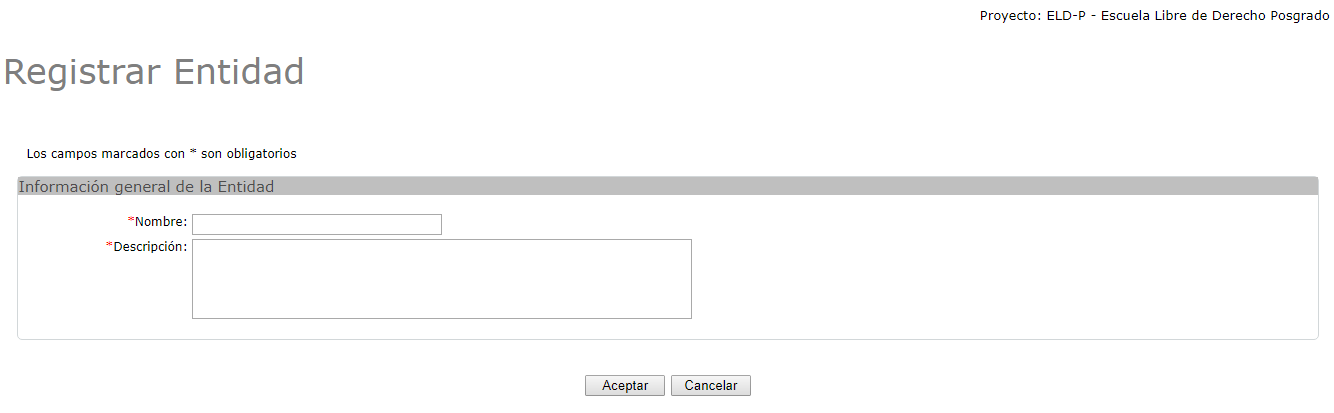
\includegraphics[scale=0.5]{roles/lider/entidades/pantallas/IU12-1registrarEntidad}
					\caption{Registrar Entidad}
					\label{fig:registrarEntidad}
				\end{center}
			\end{figure}
		
			\item Ingrese el nombre y una pequeña descripción de la entidad.
			
			\item Oprima el botón \IUAceptar.
			
			\item Se mostrará el mensaje \ref{fig:entidadRegistrada} en la pantalla \ref{fig:GestionarEntidades} ''Gestionar Entidades''.
			
			\begin{figure}[htbp!]
				\begin{center}
					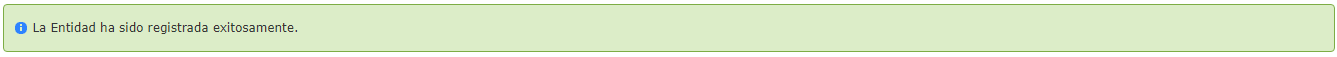
\includegraphics[scale=0.5]{roles/lider/entidades/pantallas/IU12-1MSG1}
					\caption{MSG: Entidad Registrada}
					\label{fig:entidadRegistrada}
				\end{center}
			\end{figure}
			\end{enumerate}